\chapter[Documento de Visão]{Documento de Visão}
\section{Introdução}
Esse documento tem por objetivo fornecer uma visão geral da solução de software a ser empregada para dar suporte às atividades do produto \textit{Bibliotech}. Aqui será descrito o problema a qual o software visa solucionar e dar apoio, o perfil do usuário que estará utilizando o sistema, e uma breve descrição de suas funcionalidades.

\section{Posicionamento}
Essa seção contém a descrição dos problemas, envolvidos e usuários, e subsequentemente a posição do produto.


\section{Descrição dos Problemas}
Nas figuras abaixo estão descritos os problemas identificados.

\begin{figure}[!h]
\centering
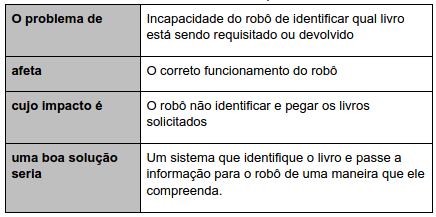
\includegraphics[scale=0.65, angle = 360]{figuras/descricao_problema1}
\caption[]{Problema 01 (fonte: Autor)}
\end{figure}
\FloatBarrier

\begin{figure}[!h]
\centering
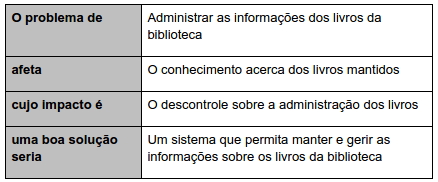
\includegraphics[scale=0.65, angle = 360]{figuras/descricao_problema2}
\caption[]{Problema 02 (fonte: Autor)}
\end{figure}
\FloatBarrier

\begin{figure}[!h]
\centering
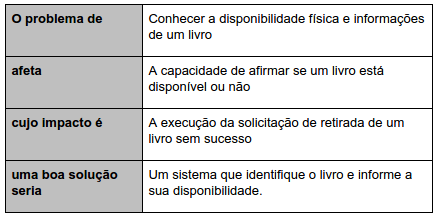
\includegraphics[scale=0.65, angle = 360]{figuras/descricao_problema3}
\caption[]{Problema 03 (fonte: Autor)}
\end{figure}
\FloatBarrier

\begin{figure}[!h]
\centering
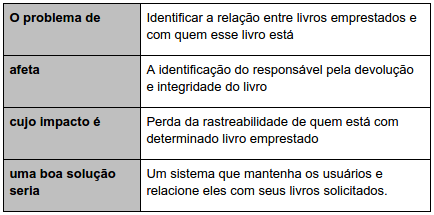
\includegraphics[scale=0.65, angle = 360]{figuras/descricao_problema4}
\caption[]{Problema 04 (fonte: Autor)}
\end{figure}
\FloatBarrier

\section{Descrições dos Usuários}
Essa seção apresenta uma descrição geral dos usuários do sistema, assim como suas respectivas responsabilidades e as suas necessidades ao utilizar o sistema.

\subsection{Resumo dos Usuários}
A a figura abaixo apresenta a descrição de cada usuário do sistema.

\begin{figure}[!h]
\centering
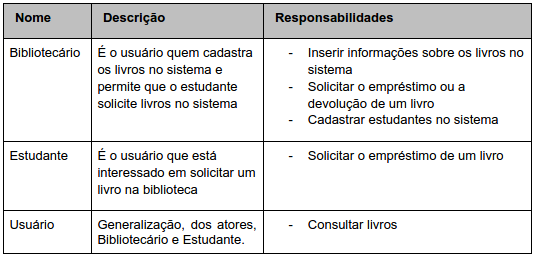
\includegraphics[scale=0.65, angle = 360]{figuras/descricao_usuarios_soft}
\caption[]{Descrição dos usuários do sistema (fonte: Autor)}
\end{figure}
\FloatBarrier

\subsection{Principais Necessidades dos Usuários}
A figura a seguir apresenta as necessidades dos usuários do sistema, a prioridade e quais são as soluções propostas para cada necessidade.

\begin{figure}[!h]
\centering
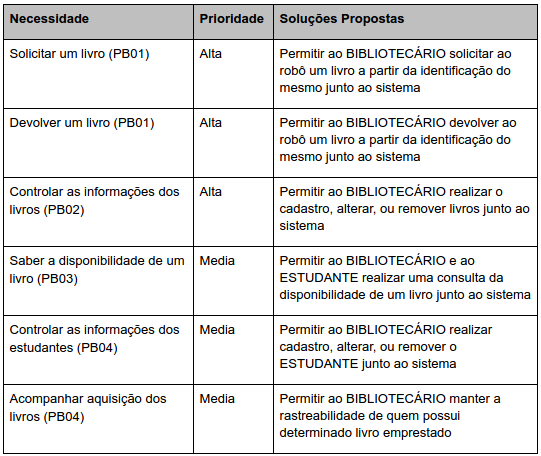
\includegraphics[scale=0.65, angle = 360]{figuras/necessidades_soft}
\caption[]{Necessidades dos usuários do sistema (fonte: Autor)}
\end{figure}
\FloatBarrier

\section{Visão Geral do Produto}
Essa seção fornece o detalhamento de como o sistema se relaciona com os outros componentes do produto.

\subsection{Perspectiva do Produto}
O sistema descrito neste documento faz parte do produto \textit{Bibliotech}. Dessa forma, ele é um subsistema e interage com outros subsistemas, a fim de atingir o objetivo final do produto.

A função do portal é implementar uma interface entre o usuário e o \textit{software} embarcado que realiza o controle das funções do robô. Para isso, ele fornece uma interface \textit{web} que permite ao bibliotecário solicitar que determinadas ações sejam executadas pelo robô. Em última instância, estas solicitações provocam a emissão de uma série de comandos para o robô.

A forma em que o sistema \textit{web} se comunica com o \textit{software} embarcado é através de uma rede \textit{wireless} local. A solicitação da realização de uma tarefa feita pelo usuário gera uma requisição ao \textit{software} embarcado que envia um código específico que indica ao \textit{software} o tipo de tarefa que o robô deve realizar. Desta forma, o \textit{software} embarcado é capaz de determinar quais funções do robô devem ser acionadas.

Após o término da tarefa do robô, o \textit{software} embarcado envia uma resposta ao sistema \textit{web} indicando o status da tarefa. Por fim, o sistema \textit{web} fornece um \textit{feedback} para o usuário indicando o status da tarefa conforme os padrões de usabilidade adotados no projeto.
